\subsection{Entitások}

%83
\begin{frame}
  Nem lehet minden karaktert közvetlenül begépelni, mert
  \begin{itemize}
    \item Böngésző félreértelmezheti, pl. \kiemel{\texttt{<}} (cimke eleje), \kiemel{\texttt{"}} (attribútum érték jelölése)
    \item ezért nem teljesíti a szabvány és a validator elvárásait sem
    \item Nincs megfelelő billentyű
  \end{itemize}
  Megoldás: HTML entitások, megadhatóak
  \begin{itemize}
    \item névvel (könnyen megjegyezhető): \texttt{\kiemel{\&}mnemonik\kiemel{;}}, pl. \texttt{\&amp;}
    \item karakterkészletbeli kódjával (jobb támogatás): 
    \begin{itemize}
      \item Tizes számrendszerben: \texttt{\kiemel{\&\#}kod\kiemel{;}}, pl. \texttt{\&\#38;}
      \item Tizenhatos számrendszerben: \texttt{\kiemel{\&\#x}hexakod\kiemel{;}}, pl. \texttt{\&\#x26;}
    \end{itemize}
  \end{itemize}
  \hiv{\href{https://dev.w3.org/html5/html-author/charref}{Referencia}}
\end{frame}

%84
\begin{frame}
  \begin{table}
    \begin{tabular}{llll}
    Kar.           & Leírás                                  & Mnemonik & Kód  \\ \hline
                   & Nem törhető szóköz (Non-Breaking SPace) & nbsp     & 160  \\
    \textless{}    & Kisebb, mint (Less Than)                & lt       & 60   \\
    \textgreater{} & Nagyobb, mint (Greater Than)            & gt       & 62   \\
    \&             & Kereskedelmi és (AMPersand)             & amp      & 38   \\
    "              & Idézőjel (QUOTe)                        & quot     & 34   \\
    \euro          & Euro                                    & euro     & 8364 \\
    \copyright     & Szerzői jogvédelem (COPYright)          & copy     & 169  \\
    $\forall$      & Minden (FOR ALL)                        & forall   & 8704 \\
    $\in$          & Eleme                                   & isin     & 8712 \\
    $A$            & Alfa                                    & Alpha    & 913  \\
    $\to$          & Jobbra (Rightwards ARRow)               & rarr     & 8594
    \end{tabular}
\end{table}
\end{frame}

%85
\begin{frame}
  \begin{columns}[c]
    \column{0.68\textwidth}
  \begin{exampleblock}{\textattachfile{entitas.html}{entitas.html}}
    \scriptsize
    \lstinputlisting[style=HTML,linerange={8-21},numbers=left,firstnumber=8]{entitas.html}
  \end{exampleblock}
    \column{0.3\textwidth}
      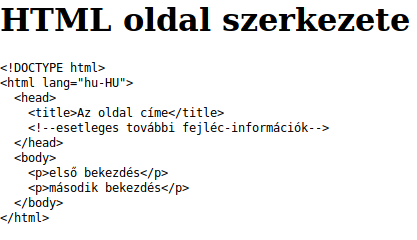
\includegraphics[width=\textwidth]{entitas.png}
  \end{columns}

\end{frame}
